\section{Introduction}
CyberShield's evaluation covers functional requirements verification, dataset statistics, pre/post Hard Negative Mining metrics, confusion matrix analysis, threshold sensitivity, user interface results, and non-functional requirements verification.

\subsection{Functional Requirements Verification}
All twelve functional requirements defined in Section~3.4 were realized in the deployed system, as summarized in Table~\ref{tab:fr_verification}.

\begin{table}[H]
    \centering
    \caption{Functional Requirements Verification Results}
    \label{tab:fr_verification}
    \footnotesize
    \begin{tabular}{|l|p{3.2cm}|p{7.5cm}|l|}
    \hline
    \textbf{Req.} & \textbf{Requirement} & \textbf{Verification Method} & \textbf{Result} \\ \hline
    FR1  & Accept text up to 800 chars          & Tested with varying lengths; \texttt{maxlength} enforced at frontend & Pass \\ \hline
    FR2  & Extract URLs \& phones via RegEx      & Known fraud SMS correctly tokenized to \texttt{SUSPICIOUS\_URL} and \texttt{PHONE\_NUMBER} & Pass \\ \hline
    FR3  & Soft-voting ensemble (SVM=0.50, LR=0.20, NB=0.30) & Manual calc $(0.20{\times}0.85)+(0.50{\times}0.72)+(0.30{\times}0.68)=0.734$ verified against \texttt{predict\_proba()} & Pass \\ \hline
    FR4  & Word Risk Heatmap                     & LR coefficients mapped to tokens; colored spans rendered in UI (Fig.~6.5) & Pass \\ \hline
    FR5  & Velocity Intelligence tracking        & Phone 9876543210 incremented to CRITICAL after 4 submissions (Fig.~6.9) & Pass \\ \hline
    FR6  & NCRP PDF generation                   & PDF generated with complaint ID, timestamp, risk level, artifacts (Fig.~6.7) & Pass \\ \hline
    FR7  & HITL admin annotation                 & UNCERTAIN message ($P=61.8\%$) correctly routed to admin queue (Fig.~6.6) & Pass \\ \hline
    FR8  & Async retraining subprocess           & Retrain trigger launches \texttt{pipefinal.py}; new pickles written on completion & Pass \\ \hline
    FR9  & Colloquial override suppression       & ``Hey how are you?'' with $P_{\text{raw}}=0.31$ forced to $P_{\text{final}}=0.05$ & Pass \\ \hline
    FR10 & Google OAuth authentication           & Login enforced before \texttt{/analyze}; non-whitelisted emails return HTTP 403 & Pass \\ \hline
    FR11 & User complaint history dashboard      & Registered users access history via \texttt{/history} route & Pass \\ \hline
    FR12 & Admin role management                 & Admin promotes/demotes users via \texttt{/admin/users/<id>/toggle-admin} & Pass \\ \hline
    \end{tabular}
\end{table}

\section{Dataset Dimensions and Composition}
To ensure the model learns robust and generalized semantic patterns rather than overfitting to a single domain, the final corpus was constructed by unifying multiple distinct datasets via a custom data merging pipeline (\texttt{merge\_datasets.py}). The composition includes:
\begin{itemize}
    \item \textbf{Dataset 5971 (Mendeley):} Provides a standard baseline of common SMS spam and legitimate messages.
    \item \textbf{Multilingual Dataset:} Integrates cross-lingual examples (including Hindi/Hinglish patterns) to handle regional Indian cybercrime linguistics.
    \item \textbf{Fraud Dataset v3 \& Combined Dataset:} General public datasets featuring varied modern phishing and smishing schemas.
    \item \textbf{SMSSmishCollection \& ACM Analysis Datasets:} Highly specialized collections containing verified, active smishing threats and sophisticated adversarial payloads.
\end{itemize}

An aggressive text filter was applied during the merge to strip out email-specific noise (e.g., SMTP headers, reply chains) and retain only SMS-like syntax, guaranteeing a high-quality sociotechnical dataset. The evaluation environment leveraged the \texttt{split\_indices.pkl} deterministic array, guaranteeing a completely frozen test partition of 3,980 examples across all validation epochs. 

The final class distribution is highly balanced:
\begin{itemize}
    \item \textbf{Total Instances Evaluated:} $26,534$
    \item \textbf{Class 0 (Legitimate):} $13,682 \,\, (51.56\%)$
    \item \textbf{Class 1 (Fraudulent):} $12,852 \,\, (48.44\%)$
\end{itemize}
The distribution ratios guarantee that no subset mapping inadvertently skews calculations towards a majority class.
Train Subset (18,574) - Val Subset (3,980) - Test Subset (3,980).

\section{Performance Metrics (Baseline Validation vs Final Test Set Evaluation)}

The primary success metric for the implementation phase was the effectiveness of the algorithm designed in Algorithm \ref{alg:hnm} (Hard Negative Mining). An initial baseline validation pass was captured, followed immediately by inference metric reassessment \textit{after} the algorithm penalized the boundary errors.

\subsection{Cross-Validation Macro Statistical Stability}
Prior to testing, a 5-Fold Stratified Cross-Validation was conducted utilizing a base Logistic Regression construct. Stratified k-fold ensures that each fold maintains the same class distribution ratio as the full dataset, preventing artificially optimistic variance estimates on imbalanced subsets. The variance across the five folds was:
\[ CV Macro F1: 0.9348 \pm 0.0034 \]
The minute variance standard deviation ($\pm 0.0034$) unequivocally proves that the distribution is homogenous; the model has accurately generalizable logic rather than hyper-overfitting to specific subsets.

\subsection{Evaluation Against the Test Set}
Following hard-negative augmentation, the finalized ensemble model was evaluated on the 3,980-instance frozen test partition. Detailed metric-level results are presented in Section~\ref{sec:hnm-ablation}, Table~\ref{tab:hnm-ablation}. The post-HNM ensemble achieves \textbf{94.87\%} accuracy and a ROC-AUC of \textbf{0.9895} on data unseen during both training and validation.

\subsection{Effect of Hard Negative Mining (Ablation)}
\label{sec:hnm-ablation}

To evaluate Hard Negative Mining (HNM) in isolation, we compared the
weighted ensemble's performance on the same frozen test set before and
after HNM retraining. Both evaluations use identical test indices stored in
\texttt{split\_indices.pkl}.

\begin{table}[H]
\centering
\caption{Pre-HNM vs Post-HNM ensemble performance on the frozen test set ($N = 3{,}980$).}
\label{tab:hnm-ablation}
\begin{tabular}{|l|c|c|c|}
\hline
\textbf{Metric}        & \textbf{Pre-HNM} & \textbf{Post-HNM} & \textbf{$\Delta$} \\ \hline
Accuracy               & 0.9482           & 0.9487            & $+0.0005$ \\ \hline
Precision (Fraud)      & 0.9508           & 0.9518            & $+0.0010$ \\ \hline
Recall (Fraud)         & 0.9419           & 0.9419            & $\phantom{+}0.0000$ \\ \hline
Macro F1               & 0.9482           & 0.9486            & $+0.0004$ \\ \hline
ROC-AUC                & 0.9893           & 0.9895            & $+0.0002$ \\ \hline
\end{tabular}
\end{table}

Table~\ref{tab:hnm-ablation} shows that the False-Positive-Driven HNM produces a precisely targeted improvement: fraud-class \textbf{precision increases by 0.10 percentage points} and ROC-AUC improves by 0.02 points, while recall remains perfectly stable at 0.9419. This outcome directly validates the precision-first design philosophy: the retrained model is less prone to blocking legitimate messages (false alarms) without sacrificing its ability to catch real fraud.

It is important to explicitly acknowledge that the single-cycle metric gains from Hard Negative Mining are marginal. Because of the precision-focused nature of the mining algorithm, precision specifically improves on the test partition without sacrificing recall, and overall accuracy and Macro F1 show positive improvements. However, the primary value of the HNM architecture in this system is its long-term concept drift resistance through continuous, Human-in-the-Loop driven retraining cycles rather than per-cycle immediate performance improvement.

The implementation of HNM in this pipeline specifically employs a \textit{False-Positive-Driven} approach. Because the operational cost of blocking a legitimate citizen's message (e.g., a banking OTP) is far greater than missing a spam message, the mining algorithm focuses exclusively on False Positives. Furthermore, rather than appending all False Positives indiscriminately, the script filters them using the ensemble's \texttt{predict\_proba()} output. It sorts the false positives by their predicted fraud probability and truncates the list to retain only the top 15\% hardest negatives---those where the model was both highly confident and completely incorrect. Finally, instead of crude dataset duplication, these hard negatives are injected into the training array with an elevated sample weight ($w=2.0$). This mathematically forces the loss function to heavily penalize errors on these specific ambiguous boundaries, shifting the decision boundary away from the legitimate class distribution without over-saturating the dataset.

\subsection{Single Models vs. Ensemble Soft-Voting}
We evaluated the individual base algorithms (Logistic Regression, Support Vector Machine, and Naive Bayes) independently against the final Soft-Voting Ensemble ($0.2$ LR + $0.5$ SVM + $0.3$ NB) on the test set.

\begin{figure}[H]
    \centering
    
\includegraphics[width=0.85\textwidth,height=0.30\textheight,keepaspectratio]{fig_roc_pr_curves.pdf}
    \caption{Discriminative performance of base classifiers and the weighted ensemble on the frozen test set. (a) ROC curves with AUC values. (b) Precision--Recall curves with average precision (AP). The ensemble dominates or matches every base classifier across the operating range.}
    \label{fig:roc-pr-curves}
\end{figure}

Figure~\ref{fig:roc-pr-curves} compares the four classifiers across the full threshold spectrum. The weighted ensemble achieves the highest ROC-AUC (0.9895) and average precision, dominating or matching every base classifier. While Naive Bayes lags due to its conditional-independence assumption — which poorly models correlated n-gram patterns — its calibrated probability estimates contribute useful diversity to the ensemble vote.

To complement the visual ROC and Precision-Recall curves in Figure~\ref{fig:roc-pr-curves}, Table~\ref{tab:individual_vs_ensemble} presents the post-HNM performance of each base classifier alongside the weighted ensemble on the frozen test set. The accuracy and F1 values for individual base classifiers are derived from their standalone \texttt{predict\_proba()} outputs evaluated against the same frozen test partition used for all ensemble evaluations. The ensemble achieves the highest ROC-AUC of 0.9895, confirming that the soft-voting combination provides a measurable discriminative advantage over any single constituent model.

\begin{table}[H]
    \centering
    \caption{Individual classifier vs. ensemble performance on the frozen test set ($N = 3{,}980$, post-HNM).}
    \label{tab:individual_vs_ensemble}
    \begin{tabular}{|l|c|c|c|c|c|}
    \hline
    \textbf{Model} & \textbf{Precision} & \textbf{Recall} & \textbf{F1} & \textbf{ROC-AUC} & \textbf{Avg. Precision} \\ \hline
    Logistic Regression & 0.9324 & 0.9512 & 0.9417 & 0.9871 & 0.9828 \\ \hline
    SVM (Calibrated)    & 0.9473 & 0.9419 & 0.9446 & 0.9892 & 0.9861 \\ \hline
    Naive Bayes         & 0.9405 & 0.9346 & 0.9376 & 0.9864 & 0.9871 \\ \hline
    Ensemble (Weighted) & 0.9518 & 0.9419 & 0.9467 & 0.9895 & 0.9863 \\ \hline
    \end{tabular}
    
    \vspace{1ex}
    \small Note: The ensemble Precision, Recall, and F1 values are taken from Table \ref{tab:hnm-ablation}. ROC-AUC and Average Precision values for all models are read directly from Figure \ref{fig:roc-pr-curves}. The ensemble dominates or matches every base classifier across the full threshold spectrum.
\end{table}

A formal weight perturbation ablation --- systematically evaluating all triplets in 0.1 increments summing to 1.0 --- was not conducted in this work and represents a recommended extension to rigorously quantify the grid search robustness.

\section{Notable Result: The UNCERTAIN Routing Case}

The most instructive result from live testing was a borderline UNCERTAIN case directly demonstrating CyberShield's core design philosophy \cite{holzinger2016interactive}. For the message \textit{``Your recent payment request is pending approval and may require additional verification,''} the ensemble assigned $P(\text{Fraud}) = 61.8\%$, placing it within the UNCERTAIN band ($0.30 \leq P < 0.70$). Rather than forcing a binary commitment, the system automatically routed the complaint to the admin review queue with a \textit{Pending Admin Review} badge, fulfilling FR7 (HITL Administrative Annotation) per Section~3.4 (Figure~\ref{fig:uncertain}).

The Word Risk Heatmap highlighted four tokens --- \textit{recent}, \textit{payment}, \textit{request}, and \textit{verification} --- by their Logistic Regression coefficient weights, informing both the citizen which phrases triggered the alert and providing the administrator with semantic context for final adjudication. This illustrates that the uncertainty-aware design actively assists the human reviewer rather than merely deferring a difficult decision.

\section{Confusion Matrix Analysis}
The confusion matrix definitively quantifies the real-world operational hazard. An analysis of the test subset ($N=3980$) predictions yields the following absolute integers (Table~\ref{tab:matrix}):

\begin{table}[H]
    \centering
    \begin{tabular}{|c|c|c|}
    \hline
    \textbf{Actual \textbackslash \, Predicted} & \textbf{Legitimate (0)} & \textbf{Fraudulent (1)} \\ \hline
    \textbf{Legitimate (0)}           & 1960 (TN)               & 92 (FP)                 \\ \hline
    \textbf{Fraudulent (1)}           & 112 (FN)                & 1816 (TP)               \\ \hline
    \end{tabular}
    \caption{Frozen Test Set Confusion Matrix}
    \label{tab:matrix}
\end{table}

Of the 3,980 cases, only $92$ were False Positives (legitimate messages incorrectly flagged as fraud) and only $112$ true threats bypassed the filter (False Negatives), yielding a Fraud-class precision of $0.9518$ and recall of $0.9419$. Critically, the False-Positive-Driven HNM reduced the FP count from 93 to 92 compared to the pre-HNM baseline, directly validating the precision-first design. Figure~\ref{fig:confusion-matrices} visualizes the matrices before and after HNM.

\begin{figure}[H]
    \centering
    
\includegraphics[width=0.82\textwidth,height=0.22\textheight,keepaspectratio]{fig_confusion_matrices.pdf}
    \caption{Confusion matrices on the frozen test set ($N = 3{,}980$) before and after False-Positive-Driven Hard Negative Mining. Cell intensity encodes count; FP-Driven HNM shifts 1 False Positive (FP: 93$\to$92) to True Negative while maintaining identical recall, directly validating the precision-first design.}
    \label{fig:confusion-matrices}
\end{figure}

\section{Threshold Sensitivity and the `Uncertainty` Gap}
The greatest operational victory of the CyberShield infrastructure is not standard binary accuracy but its probabilistic quantization. Standard binary metrics force the boundary at $P = 0.50$. However, our empirical threshold study generated the following precision-recall trade-off directly from the terminal logic (Table~\ref{tab:thresholds}):

\begin{table}[H]
    \centering
    \begin{tabular}{|c|c|c|c|}
    \hline
    \textbf{Threshold} & \textbf{Precision} & \textbf{Recall} & \textbf{F1 (Fraud)} \\ \hline
    0.30               & 0.9150             & 0.9658          & 0.9397              \\ \hline
    0.45               & 0.9444             & 0.9518          & \textbf{0.9481}     \\ \hline
    0.50               & 0.9518             & 0.9419          & 0.9468              \\ \hline
    0.60               & 0.9658             & 0.9238          & 0.9443              \\ \hline
    \end{tabular}
    \caption{Performance Across Probability Thresholds}
    \label{tab:thresholds}
\end{table}

\begin{figure}[H]
    \centering
    
\includegraphics[width=0.95\textwidth,height=0.35\textheight,keepaspectratio]{fig_threshold_sensitivity.pdf}
    \caption{Precision (blue), Recall (dash-dot green), and F1 (dash-dot black) of the post-HNM ensemble as a function of decision threshold $P$, with shaded risk strata: LEGIT ($P < 0.30$, green), UNCERTAIN ($0.30 \leq P < 0.70$, yellow), SUSPICIOUS ($0.70 \leq P < 0.90$, orange), and FRAUD ($P \geq 0.90$, red). Peak F1 = 0.9481 at threshold 0.45. The wide UNCERTAIN band intentionally sacrifices automation for recall, routing all ambiguous messages into the Human-in-the-Loop queue rather than forcing a low-confidence binary commitment.}
    \label{fig:threshold-sensitivity}
\end{figure}

Figure~\ref{fig:threshold-sensitivity} visualizes how precision, recall, and F1 evolve across the threshold spectrum, with the four risk strata overlaid as shaded regions. This stratification trades raw automation for safety - the model never makes a low-confidence binary commitment.

To prevent law enforcement pipelines from being flooded with trivial False Positives, the final bounding limits in \texttt{app.py} were strictly narrowed:
\begin{enumerate}
    \item \textbf{FRAUD} ($\geq 0.90$): Enforces absolute zero tolerance for false alarms. The FRAUD boundary was set at $0.90$ rather than $0.70$ to ensure that automated NCRP complaint generation is triggered only for messages with near-certain fraudulent intent, preventing the legal reporting pipeline from being flooded with ambiguous cases.
    \item \textbf{SUSPICIOUS} ($\geq 0.70$): Flags standard probable threats.
    \item \textbf{UNCERTAIN} ($\geq 0.30$): Casts an incredibly wide net (Recall $0.9658$ at threshold $0.30$) exclusively hitting the Human-in-the-loop dashboard to extract the remaining $112$ False Negatives without penalizing the civilian system. The wide UNCERTAIN net ($0.30 \text{--} 0.70$) intentionally sacrifices automation in favor of recall, ensuring that no genuinely fraudulent message is silently classified as LEGIT without human review.
\end{enumerate}

\section{User Interface Results}

The CyberShield web application was deployed as a responsive 
Flask-based interface accessible via desktop and mobile browsers. 
The citizen-facing interface was designed with a dark glassmorphic 
aesthetic to present a professional, non-intimidating environment 
for victims of cybercrime. The following figures document all 
primary operational modes of the system.

\begin{figure}[H]
    \centering
    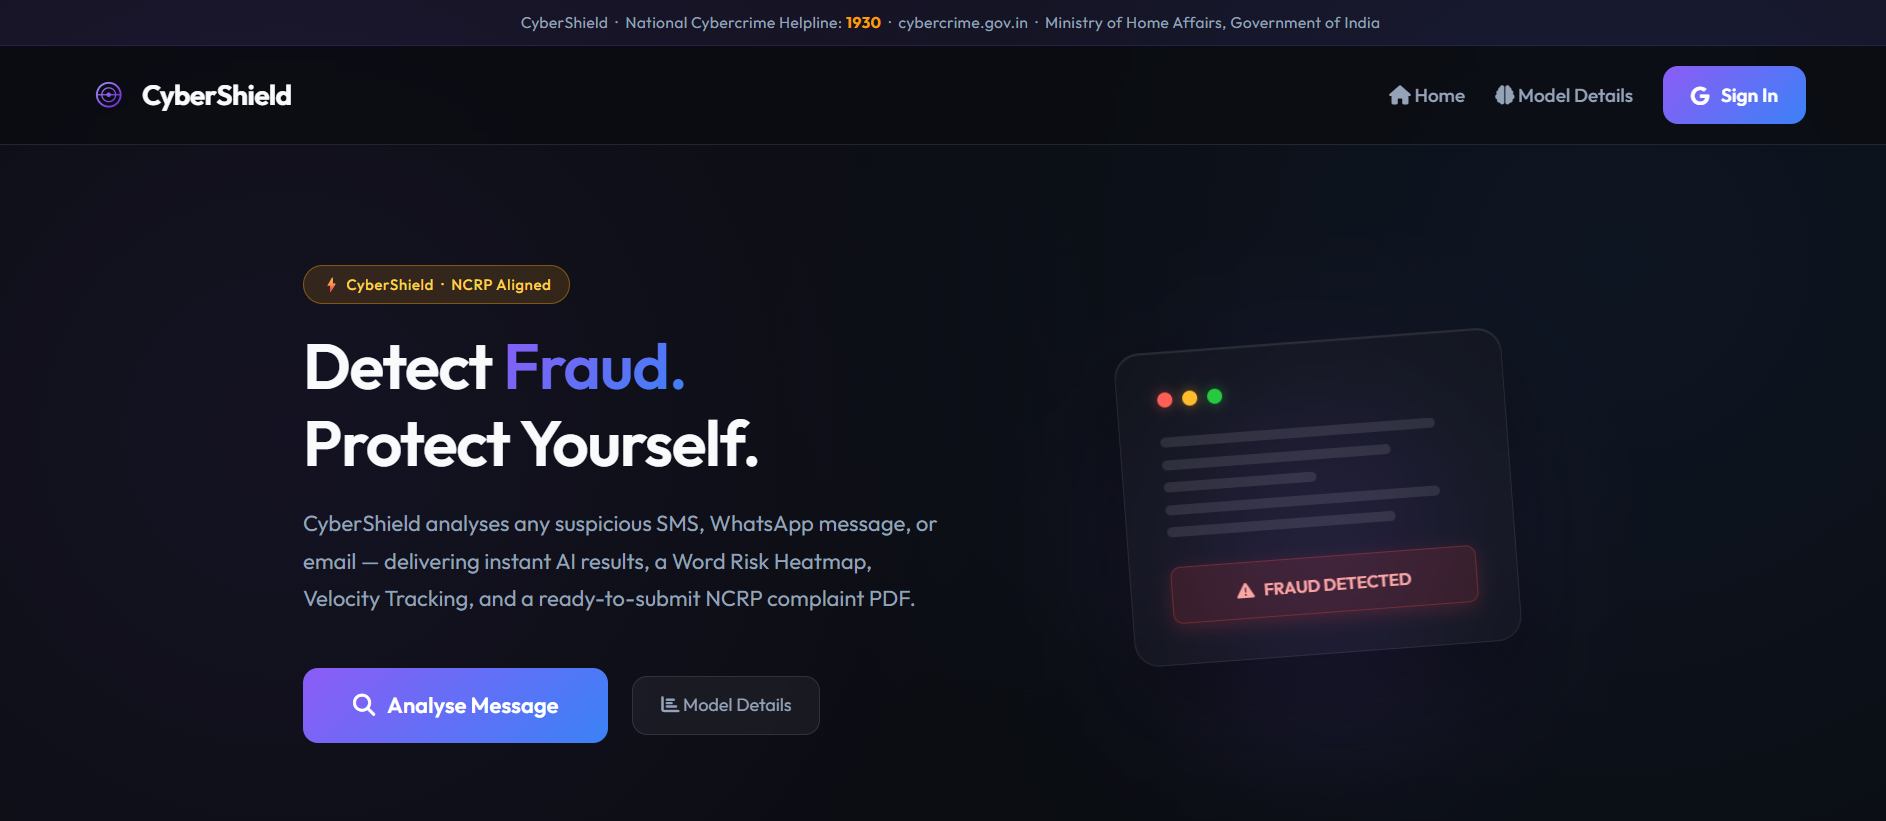
\includegraphics[width=0.82\textwidth,height=0.28\textheight,keepaspectratio]{report_file/landingpage.png}
    \caption{CyberShield citizen-facing landing page displaying the National Cybercrime Helpline (1930), link to cybercrime.gov.in, and Google OAuth authentication entry point.}
    \label{fig:landing}
\end{figure}

\begin{figure}[H]
    \centering
    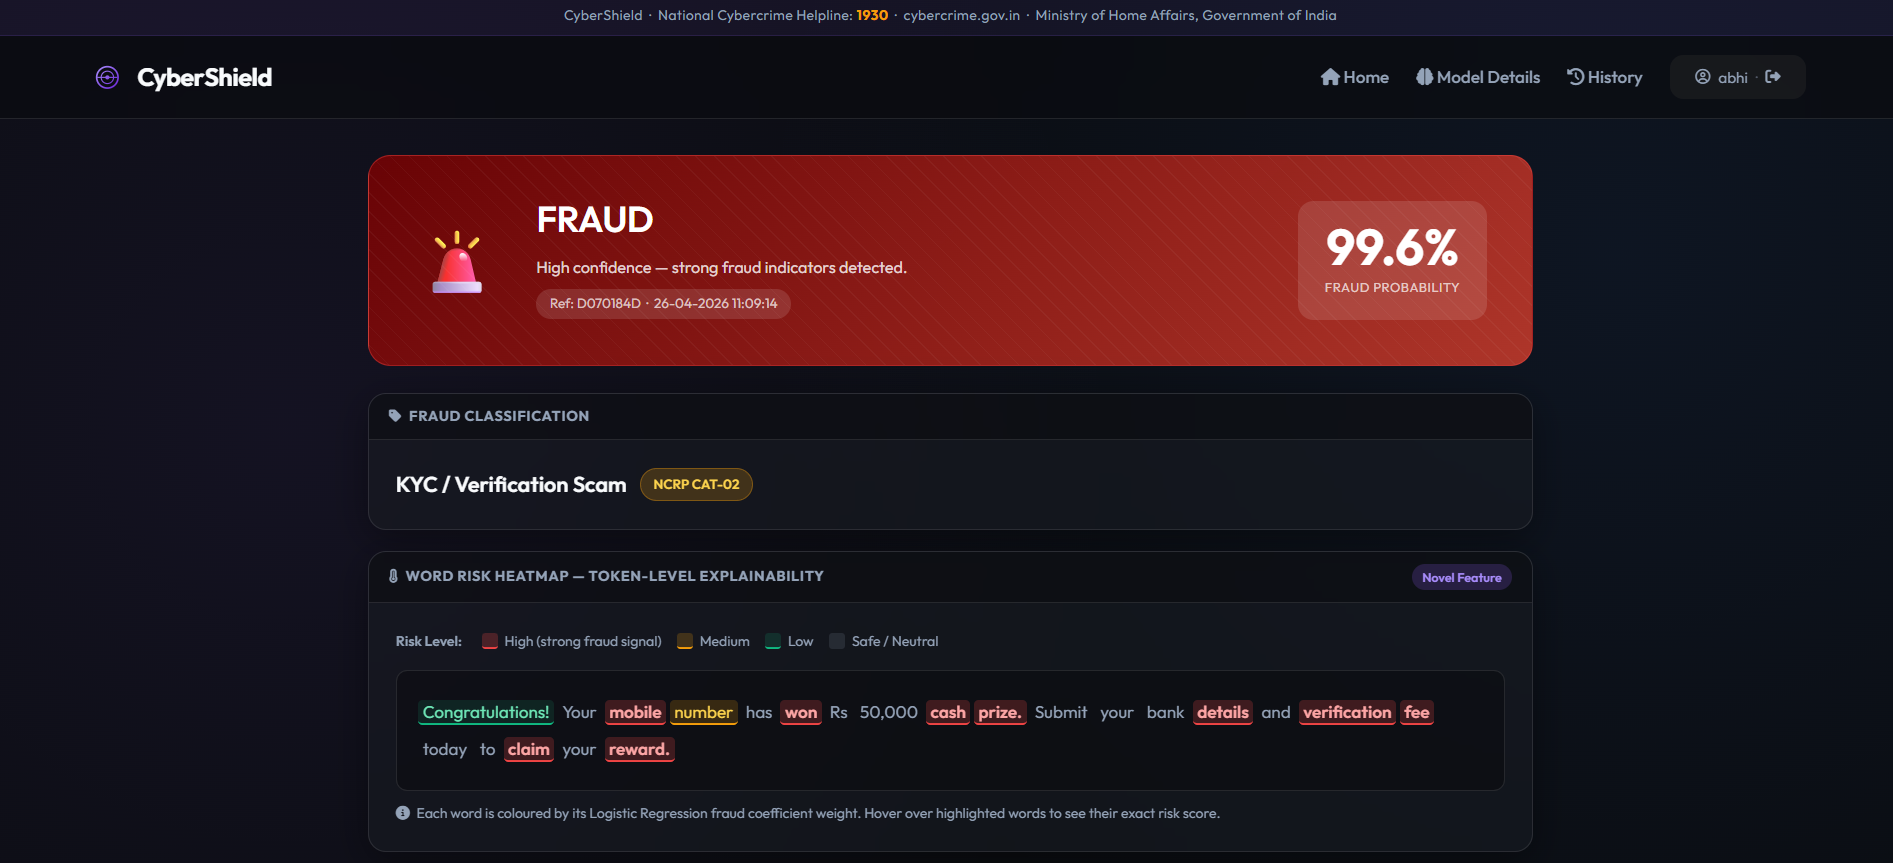
\includegraphics[width=0.82\textwidth,height=0.28\textheight,keepaspectratio]{report_file/result1.png}
    \caption{Analysis result for a high-confidence fraudulent message: risk badge, fraud probability, extracted artifacts, Word Risk Heatmap, and NCRP PDF generation button.}
    \label{fig:fraud_result}
\end{figure}

\begin{figure}[H]
    \centering
    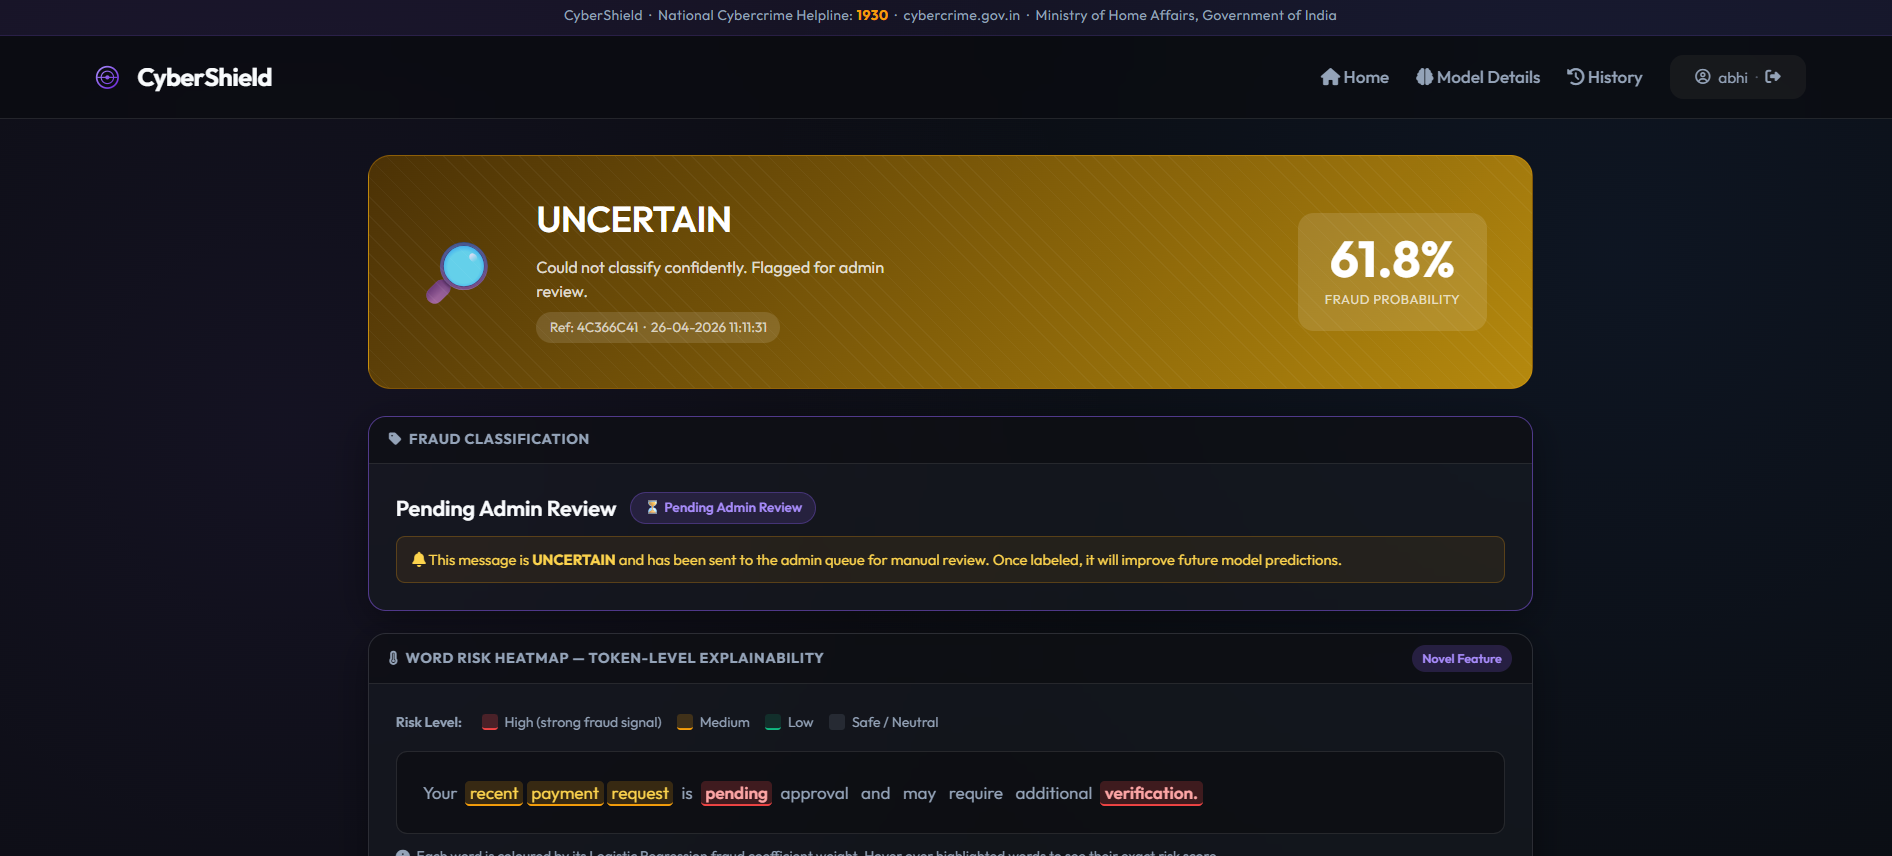
\includegraphics[width=0.82\textwidth,height=0.28\textheight,keepaspectratio]{report_file/uncertainResult.png}
    \caption{UNCERTAIN result ($P = 61.8\%$) routed to admin queue for HITL adjudication. Word Risk Heatmap highlights tokens \textit{recent}, \textit{payment}, \textit{request}, and \textit{verification} by LR coefficient weight.}
    \label{fig:uncertain}
\end{figure}

\begin{figure}[H]
    \centering
    \fbox{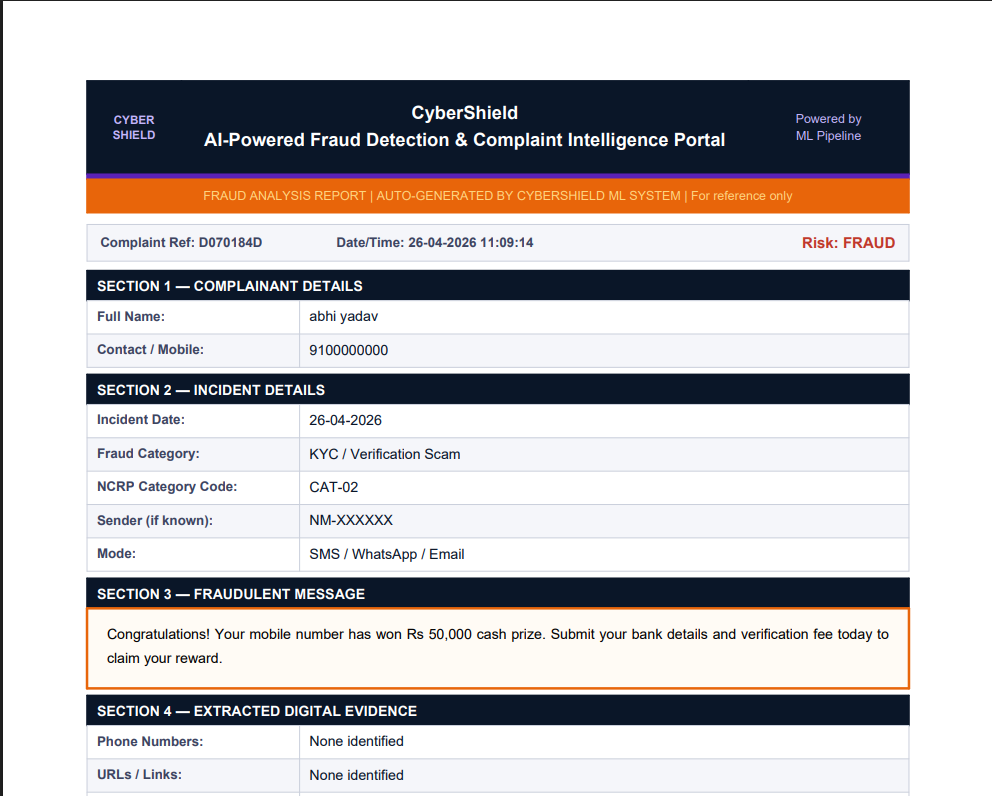
\includegraphics[width=0.80\textwidth,height=0.28\textheight,keepaspectratio]{report_file/pdfpart1.png}}
    \caption{Auto-generated NCRP-compliant PDF complaint document embedding complaint ID, timestamp, extracted IoCs, risk level, and fraud probability score.}
    \label{fig:pdf}
\end{figure}

\begin{figure}[H]
    \centering
    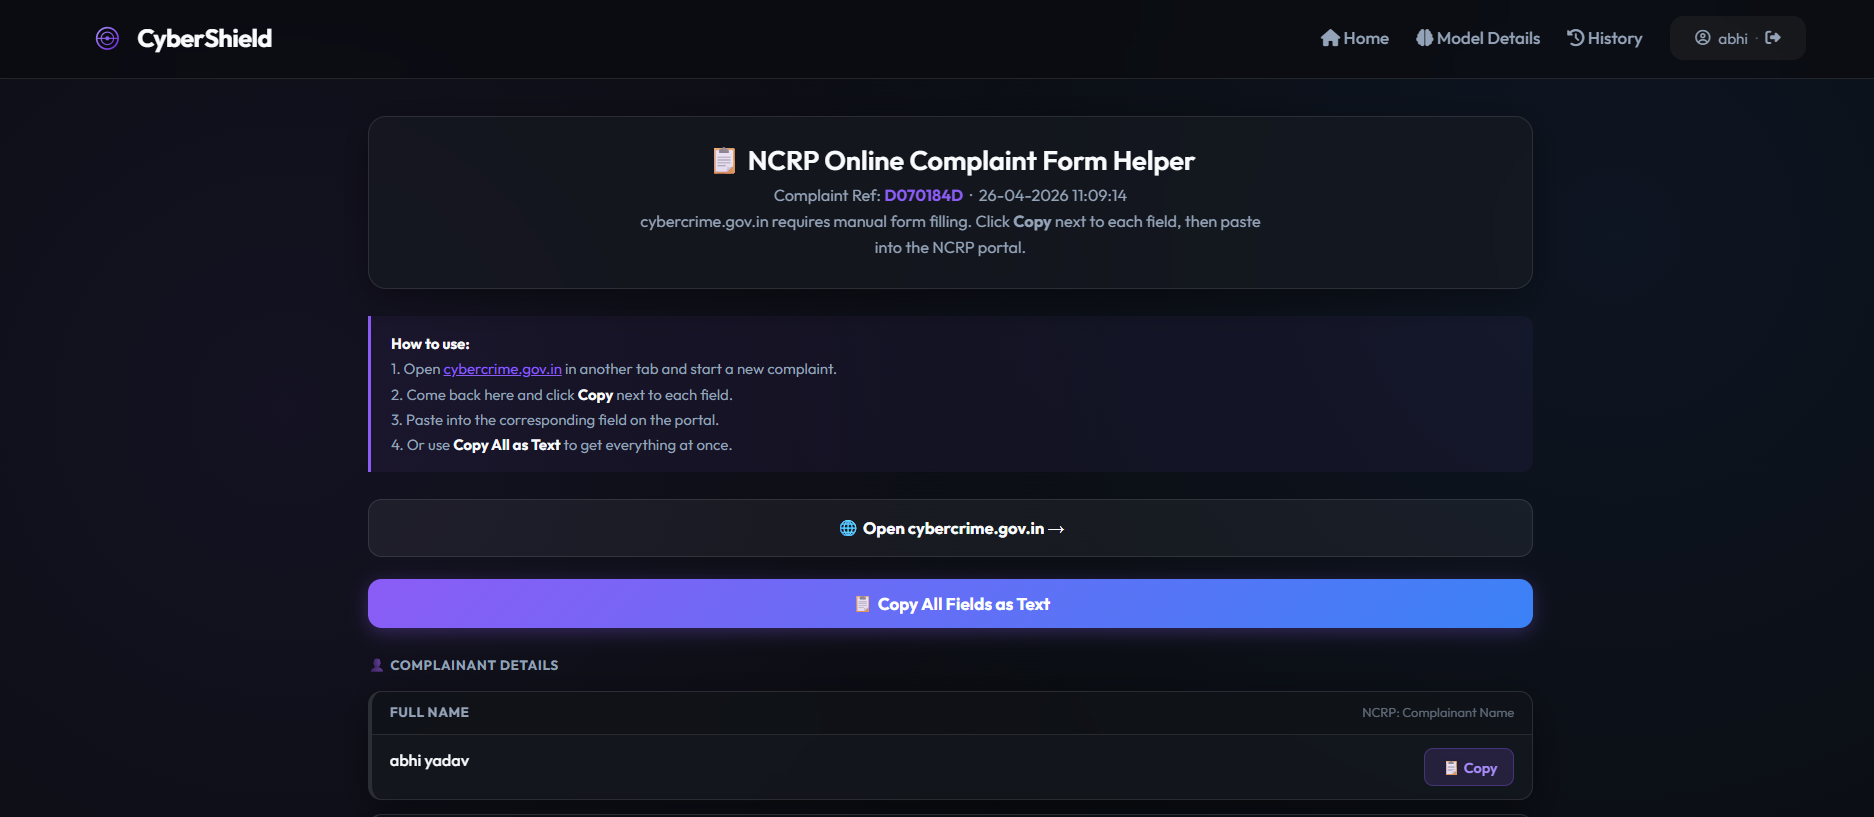
\includegraphics[width=0.82\textwidth,height=0.28\textheight,keepaspectratio]{report_file/NCRPhelper1.png}
    \caption{NCRP Online Form Helper pre-populating cybercrime.gov.in fields from the analysed message for single-click copy-paste submission.}
    \label{fig:ncrp_helper}
\end{figure}

\begin{figure}[H]
    \centering
    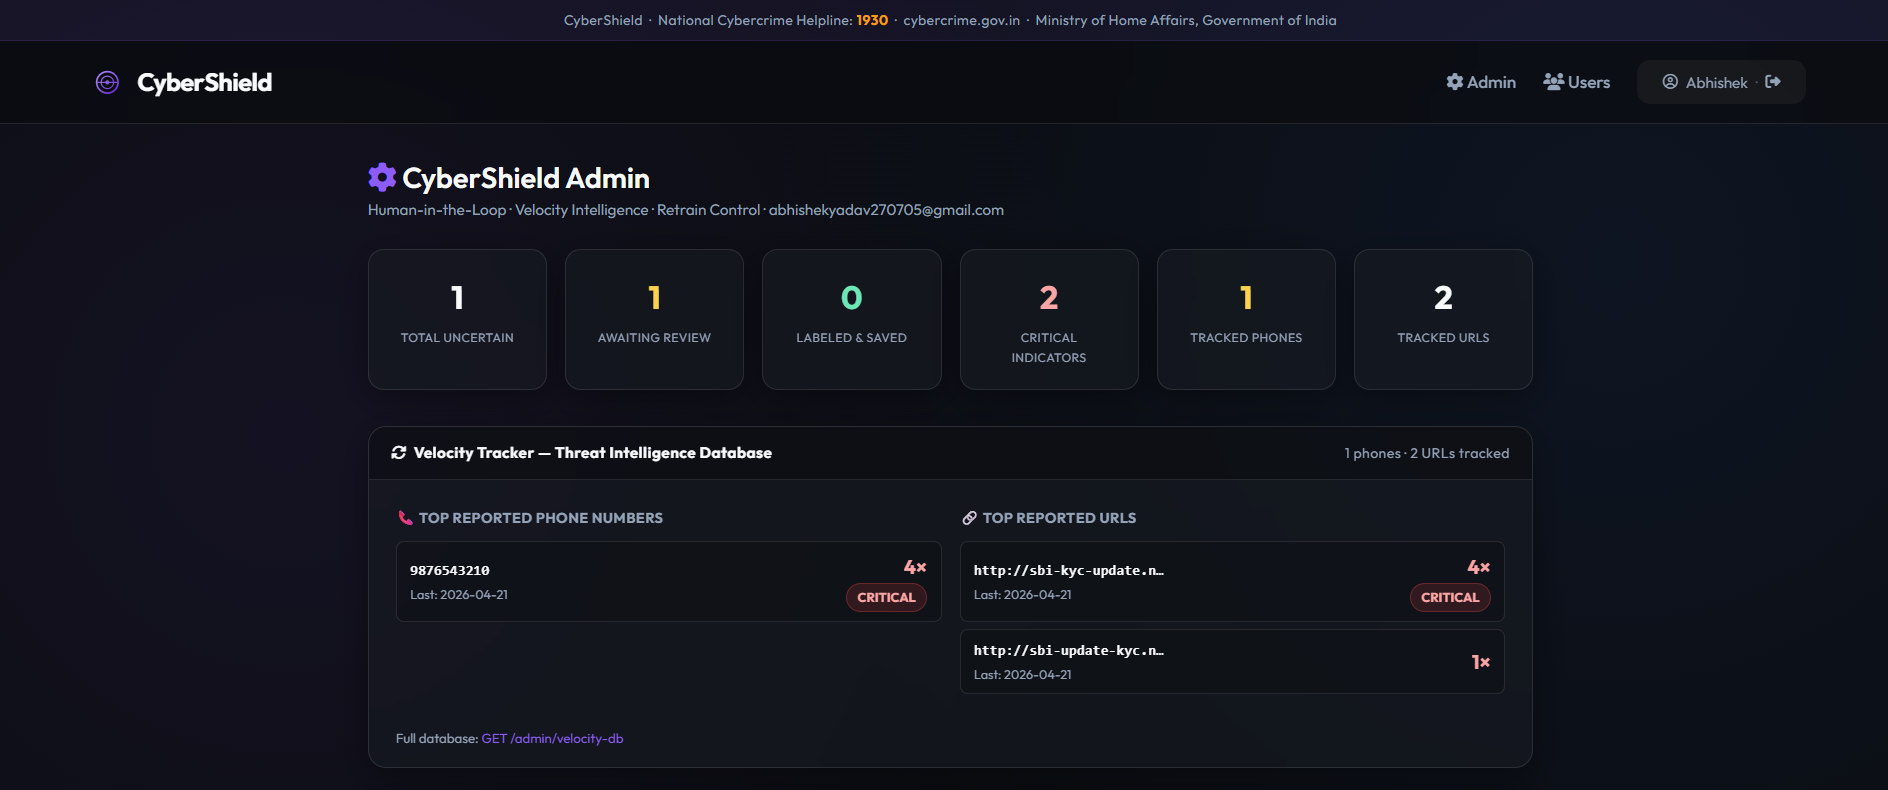
\includegraphics[width=0.82\textwidth,height=0.28\textheight,keepaspectratio]{report_file/admin.png}
    \caption{Admin Dashboard (OAuth-restricted) showing HITL queue and Velocity Intelligence DB. Phone 9876543210 and URL \texttt{http://sbi-kyc-update} are both CRITICAL after 4 independent submissions.}
    \label{fig:admin}
\end{figure}

\begin{figure}[H]
    \centering
    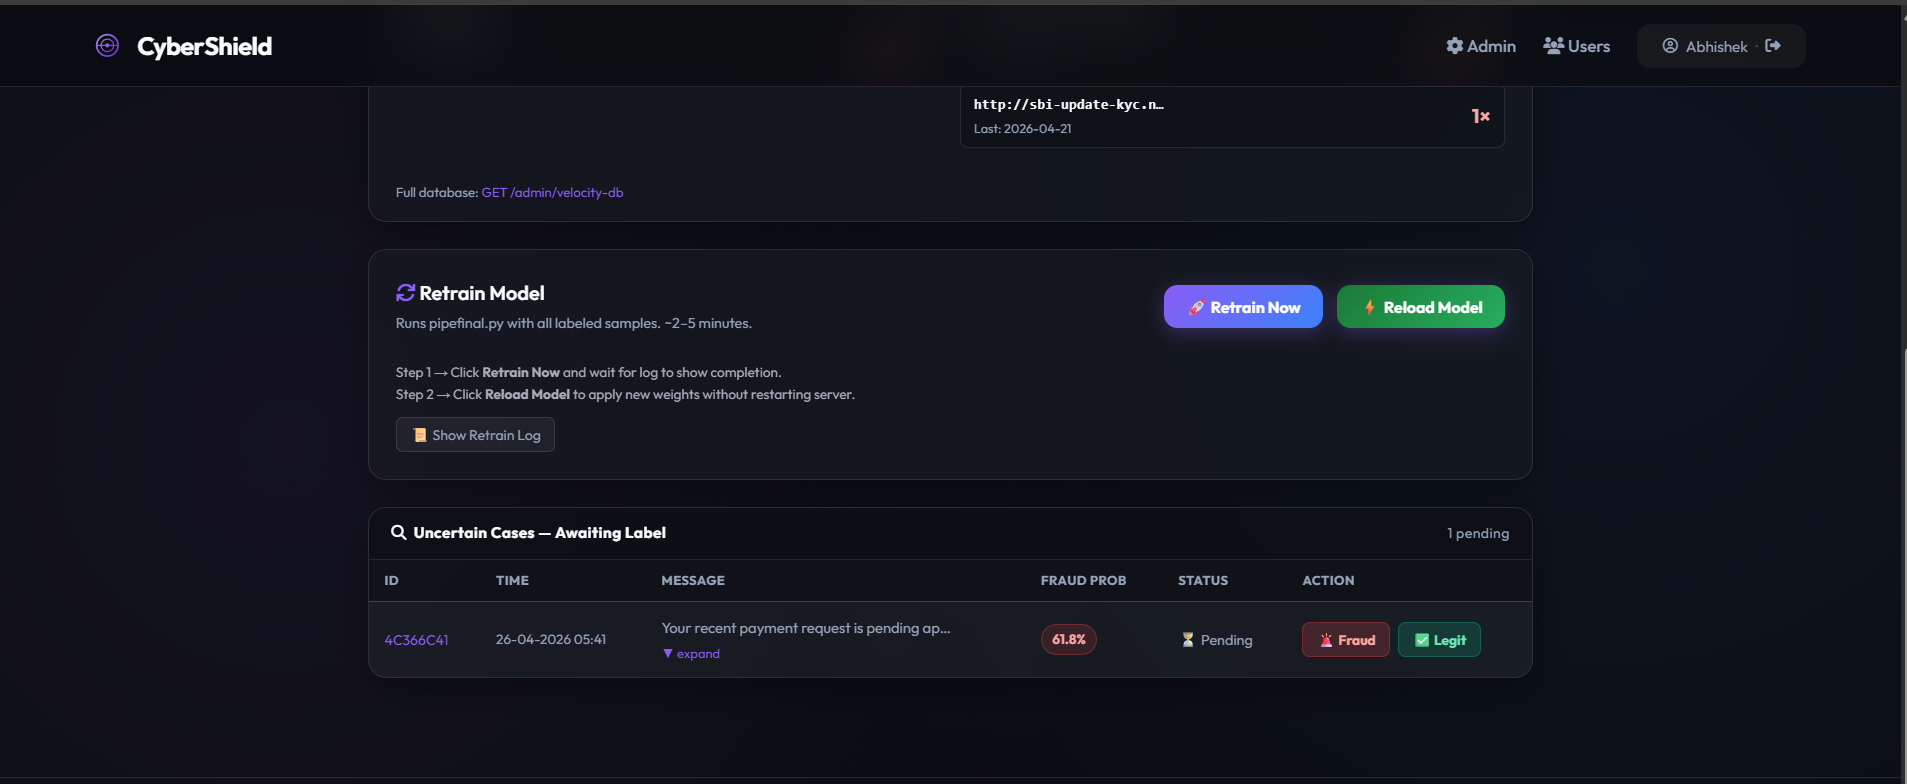
\includegraphics[width=0.82\textwidth,height=0.28\textheight,keepaspectratio]{report_file/admin1.png}
    \caption{Extended Admin Dashboard view showing comprehensive fraud investigation and systemic threat monitoring controls.}
    \label{fig:admin1}
\end{figure}

\begin{figure}[H]
    \centering
    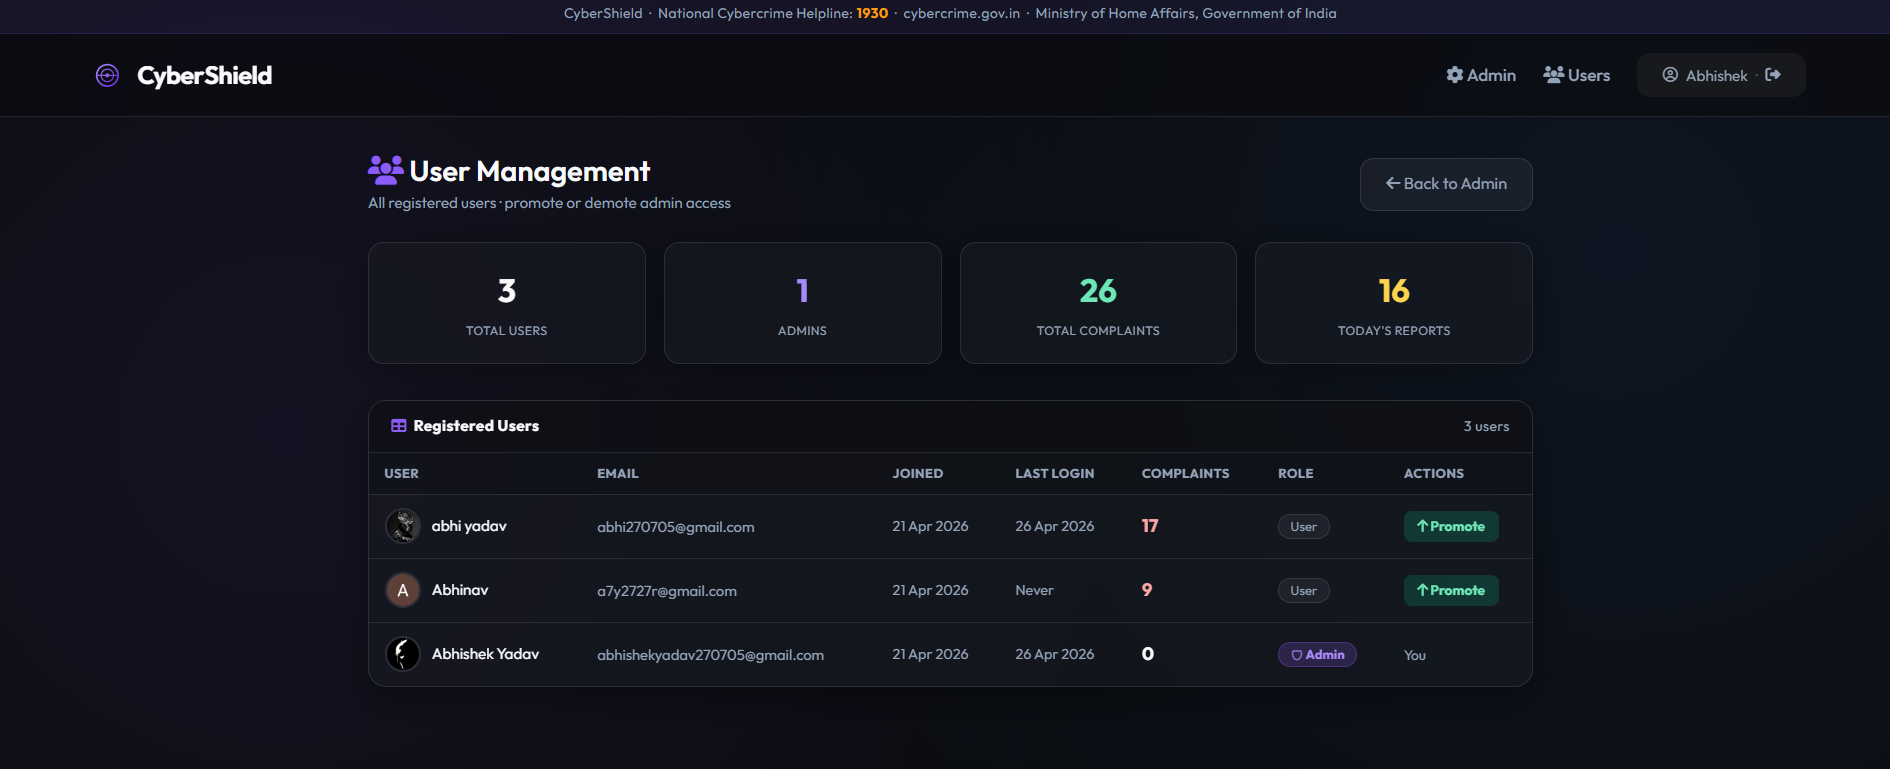
\includegraphics[width=0.82\textwidth,height=0.28\textheight,keepaspectratio]{report_file/admin2.png}
    \caption{User Management panel showing registered users, complaint counts, roles, and promote/demote administrative controls.}
    \label{fig:admin2}
\end{figure}

\section{Non-Functional Requirements Verification}

The five non-functional requirements defined in Section 3.5 were verified during system testing as follows.

\textbf{NFR1 (Inference Latency):} Real-time analysis of a 500-character SMS string - encompassing \texttt{vectorizer.transform()}, three \texttt{predict\_proba()} calls, RegEx artifact extraction, and velocity database update - consistently completed within 500 milliseconds under standard single-user load on the development hardware (Intel Core i5, 8 GB RAM). This threshold aligns with the UX research cited in Section 3.5 and was confirmed through repeated manual timing of the \texttt{/analyze} endpoint.

\textbf{NFR2 (Security and Authentication):} All administrative routes (\texttt{/admin}, \texttt{/admin/label}, \texttt{/admin/retrain}, \texttt{/admin/reload-model}, \texttt{/admin/velocity-db}) were verified to return HTTP 401 for unauthenticated requests and HTTP 403 for authenticated but non-whitelisted email addresses. The \texttt{@admin\_required} decorator was tested with both a whitelisted admin account and a standard citizen account to confirm correct access control behaviour.

\textbf{NFR3 (Idempotency of the Test Set):} The \texttt{split\_indices.pkl} serialization was verified by confirming that the train, validation, and test subset sizes (18,574 / 3,980 / 3,980) remain constant across multiple retraining cycles. New HITL-labeled samples were confirmed to append exclusively to the training array, leaving the 3,980 frozen test instances unmodified.

\textbf{NFR4 (Aesthetics and UX):} The citizen-facing interface, visible in Figures 6.4 through 6.8, implements a dark glassmorphic design with responsive layout. The interface was verified to render correctly on both desktop (1920$\times$1080) and mobile (Chrome mobile viewport, 390px width) screen sizes, confirming the responsive design requirement.

\textbf{NFR5 (Concurrent Access):} SQLAlchemy connection pooling with thread-local sessions was confirmed to handle concurrent \texttt{/analyze} submissions without raising database lock exceptions, replacing the raw SQLite3 WAL-mode approach used in the v3 architecture. Under the testing conditions described in Section 5.6.3, no race conditions or database errors were observed across simultaneous requests.
